\documentclass[]{IEEEtran}
\usepackage[utf8]{inputenc}		%UTF8 input file
\usepackage[T1]{fontenc}		
\usepackage[ngerman]{babel}
\usepackage{amsmath, amssymb}
\usepackage{eurosym}
%Für Fußzeilten
%\usepackage{stfloats}
%Bilder
\usepackage{graphicx}

%Zeilenabstände
\usepackage{setspace}


\title{Pflanzengießanlage}
%\subtitle{DIY14Pflanze}
\date{\today}
\author{ Stefan Schubäck, \and Matthias Nagl,\and Christoph Hofbauer, \and Dmitrii Cetvericov, \and Markus Fischer-Has,}

%\renewcommand{\iedlistdecl}{\settowidth{\labelwidth}{Hello}}

\begin{document}


	\maketitle
%	\tableofcontents


\section{Idee}\label{refIdee}
Auch unter den Studenten gibt es den einen oder anderen mit einem grünen Daumen, der seine WG will durch ein paar Pflanzen aufgewertet hat. Wenn nur nicht das ständige Gießen wäre. Vor jedem längeren Urlaub stellt sich die Frage, was machen mit den ganzen Pflanzen? Den Nachbarn fragen und hoffen er ist da und verlässlich. Die Pflanzen "Absaufen" lassen und hoffen, dass die sich das was einteilen? Beides keine zufriedenstellende Lösung. Wieso lässt man sich die Pflanze nicht selber gießen?

Aus diesen Überlegungen ist die Idee entstanden, eine Pflanze mit Sensoren auszustatten, die uns über den aktuellen Zustand Informieren. Die wichtigste Information in dieser Hinsicht ist natürlich die Bodenfeuchtigkeit im Topf der Pflanze. Neben dieser können noch weitere Informationsquellen herangezogen werden, die über das Wohlbefinden der Pflanze Aufschluss geben. Hierunter fallen unter anderer der Nährstoffgehalt der Erde, die Temperatur an der Wurzel oder die Luftqualität im Umfeld der Pflanze.

Gießsystem WG


\section{Eingrenzung}
Im Rahmen des Projekts soll ein Gießsystem für eine alleinstehende Pflanze erstellt werden. Es misst die Bodenfeuchtigkeit der Pflanze gießt und bei bedarf die Pflanze. Das Wasser hierfür wird mithilfe einer Pumpe aus einem bereitgestellten Wassertank entnommen. Das System ist für den Innenraum ausgelegt und soll autonom ohne das Zutun des Menschen die Pflanze gießen. Der notwendige Strom wird über ein Netzteil bereitgestellt. Als Zusatzfeature soll das Gießsystem seine Messwerte Drahtlos an einen Computer übermitteln.
 
Weitere Ideen wie z.B. eine Autarke Lösung mit Batterien, ein \emph{Mehr-Pflanzenbetrieb} oder ein System für den Garten wurden zwar diskutiert aber wegen dem erhörten Zeitaufwand und begrenzten Budgets nicht weiter verfolgt. Auch wurde auf ein Warnsystem verzichtet, der den Menschen informiert, dass der Wassertank leer wird. 


\section{Mechanik}
Das System lässt sich in drei Bereiche einteilen. Zum ersten der Mechanik mit Hilfe der das Wasser zu der Pflanze kommt. Eine Elektronik die die Energieversorgung regelt und Messwerte aufnimmt. Gesteuert wird das ganze durch die Logik die auf ein Arduino kompatiblem Board programmiert wird.
\subsection{Wassertransport und Gefäß}
Um den Einsatzbereich so flexibel wie möglich zu halten haben wir uns für ein Pumpensystem entschieden. Dadurch ist die Anordnung der Pflanze relativ zum Wassertank nicht relevant. Der hiermit einhergehen erhöhte Strombedarf ist zu verkraften, da unser System nicht auf Batterien angewiesen ist.
	
Für den Wassertransport haben wir uns für eine Zahnradpumpe entschieden.
Diese setzte sich gegenüber anderen Lösungen vor allem wegen ihrer selbstsaugenden Eigenschaft durch.
Selbstsaugend bedeutet, dass eine mit Luft gefüllten Wasserleitung und Pumpe Wasser ansaugen und fördern kann. Als Alternativen wurden Ventile und Kreiselpumpen angedacht.
Die Kreiselpumpe konnte trotz dem geringeren Stromverbrauch und geringerem Geräuschpegel nicht durchsetzen. 
Noch weniger Strom und Lärm verursachen Ventile, die aber auf gespeicherte Energie angewiesen sind.  Entweder durch Druck im Wassertank oder durch Erhöhung des Tankes über den Ausfluss. 
Auf Grund der Wahl der Zahnradpumpe kann ein 4 mm Schlauch zur Förderung des Wassers genutzt werden. Das Gefäß ist frei wählbar deswegen wurde hier ein fünf-Liter-Weinballon gewählt. 
 In den der Schlauch gesteckt wird. Auf der anderen Seite wird das Schlauchende mit einem durchbohrten Kantholz in der Pflanzenerde befestigt.
	
	Die Nachteile der Zahnradpumpe (Stromverbrauch und Lärm) haben wir dadurch minimiert, dass das Gießsystem über ein Netzgerät mit Strom versorgt wird ist der erhöhte Stromverbrauch zwar unschön aber vertretbar. Um den Geräuschpegel zu minimieren wird über einen Helligkeitssensor verhindert, dass in der Nacht gegossen wird. Dies wird im Abschnitt~\ref{sensorik} näher erläutert.
	
\begin{table*}
	\centering
	\onehalfspacing
	
		\begin{tabular}{|l|lll|}
		\hline
		\textit{Eigenschaft} & \textit{Zahnradpumpe} & \textit{Kreiselpumpe} & \textit{Ventil} \\
		\hline
		Selbstsaugend	&ja	&nein &nein\\
		
		Lautstärke		&sehr laut	&mittel laut	&leises Klacken\\
		
		Stromverbauch	&@12V 2,8A	&@12V 0,6A	&@12V 80mA\\
		
		Förderleistung	&gering		&groß		&keine eigene\\
		
		Preis			&2,95 \euro	& 2,95 \euro	&	4,95 \euro\\
		\hline		
		\end{tabular}
		
	\caption{Vergleich Wasserpumpen und Ventil}
	\label{Vergleich zwischen Wasserpumpen und Ventil}

\end{table*}	
	
	
	
	\subsection{Gehäuse}
	Das Gehäuse wurde möglichst klein, aber genügend Platz für die Elektronik konzipiert.
	So muss es genügend Platz bieten um ein LCD-Display, zwei Taster, die Hauptplatine, das Arduino Board,  die Vorschaltung für den Bodenfeuchtesensor, die Verkabelung und Anschlüsse für die Sensoren, den Motor und Stromversorgung  bieten.
	Um den Körper der Box zu gestalten, wurde der BoxMaker benutzt und mit Inkscape angepasst. 
	Das gesamte Gehäuse wurde im FabLab Erlangen mit Hilfe des Lasercutters gefertigt.
	
\section{Elektronik}
	Im folgenden wird der Aufbau der Version 1.0 vorgestellt. Während des Aufbaus, vor allem aber während der Testphase sind ein paar Probleme aufgetreten die dazu geführt habe, dass eine neue Version 1.1 erstellt werden muss. 
	Diese neue Version ist jedoch aus zeitlichen Gründen noch nicht komplett aufgebaut. 
	Es wurden ein neues Layout erstellt und die Software bereits so angepasst, dass diese ohne größere Änderungen übernommen werden kann. 
	Im folgenden wird die Funktionsweise auf Basis der Version 1.0 erläutert, an gegebener Stelle wird auf die  Anpassungen eingegangen die bereits umgesetzt wurden bzw. noch in Planung sind. 
\begin{figure*}
	\centering
	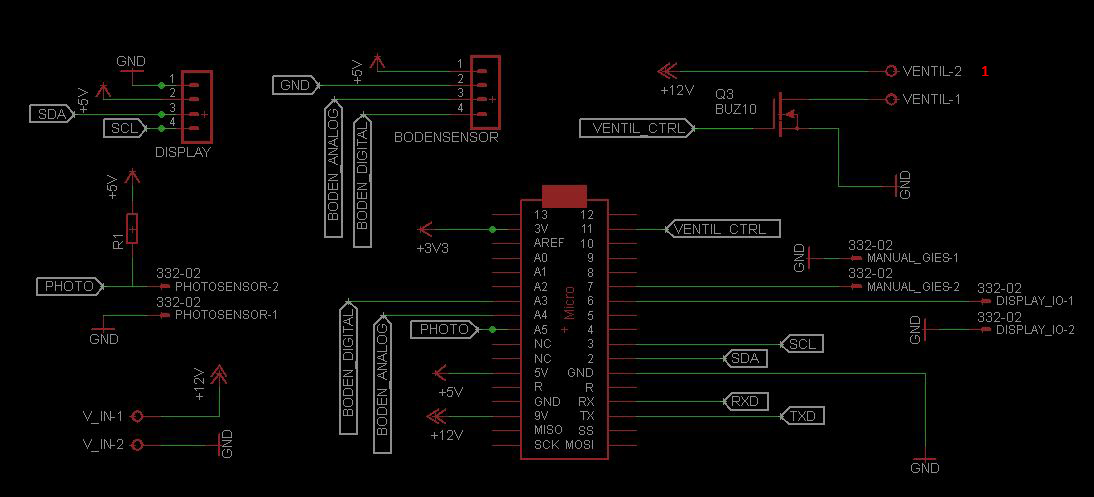
\includegraphics[width=0.9\linewidth]{bilder/v1SchaltplanMicro0.JPG}
	\caption{Schaltpaln V1.0 mit Arduino Micro}
	\label{fig-Schaltplanv1.0}
\end{figure*}

\subsection{Hauptplatine}



In Abbildung \ref{fig-Schaltplanv1.0} ist die Version 1.0 des Layouts und des Schaltplans zu sehen. Die drei Funktionsblöcke
\begin{itemize}
		\item Senorschaltung
		\item Kommunikationsschaltung
		\item Stromversorung
\end{itemize}
werden im folgenden erläutert. 
		
			
\subsubsection{Senorschaltung} \label{sensorik}
Für den Helligkeitssensor wird ein einfacher Photo-widerstand verwendet, der über einen Spannungsteiler an einem der Analogen Pins des Arduino Bords angeschlossen ist. Der Pin verfügt über einen 10Bit AD Konverter und gibt demnach einen Integerwert von 0 - 1023 zurück.
Der Bodenfeuchtesensor bestimmt den Wassergehalt des Bodens über eine Widerstandsmessung zwischen den zwei Zinken einer Messgabel. Je mehr Wasser im Erdreich vorhanden ist, desto kleiner ist der gemessene Widerstand im Boden.

\begin{figure}
	\centering
	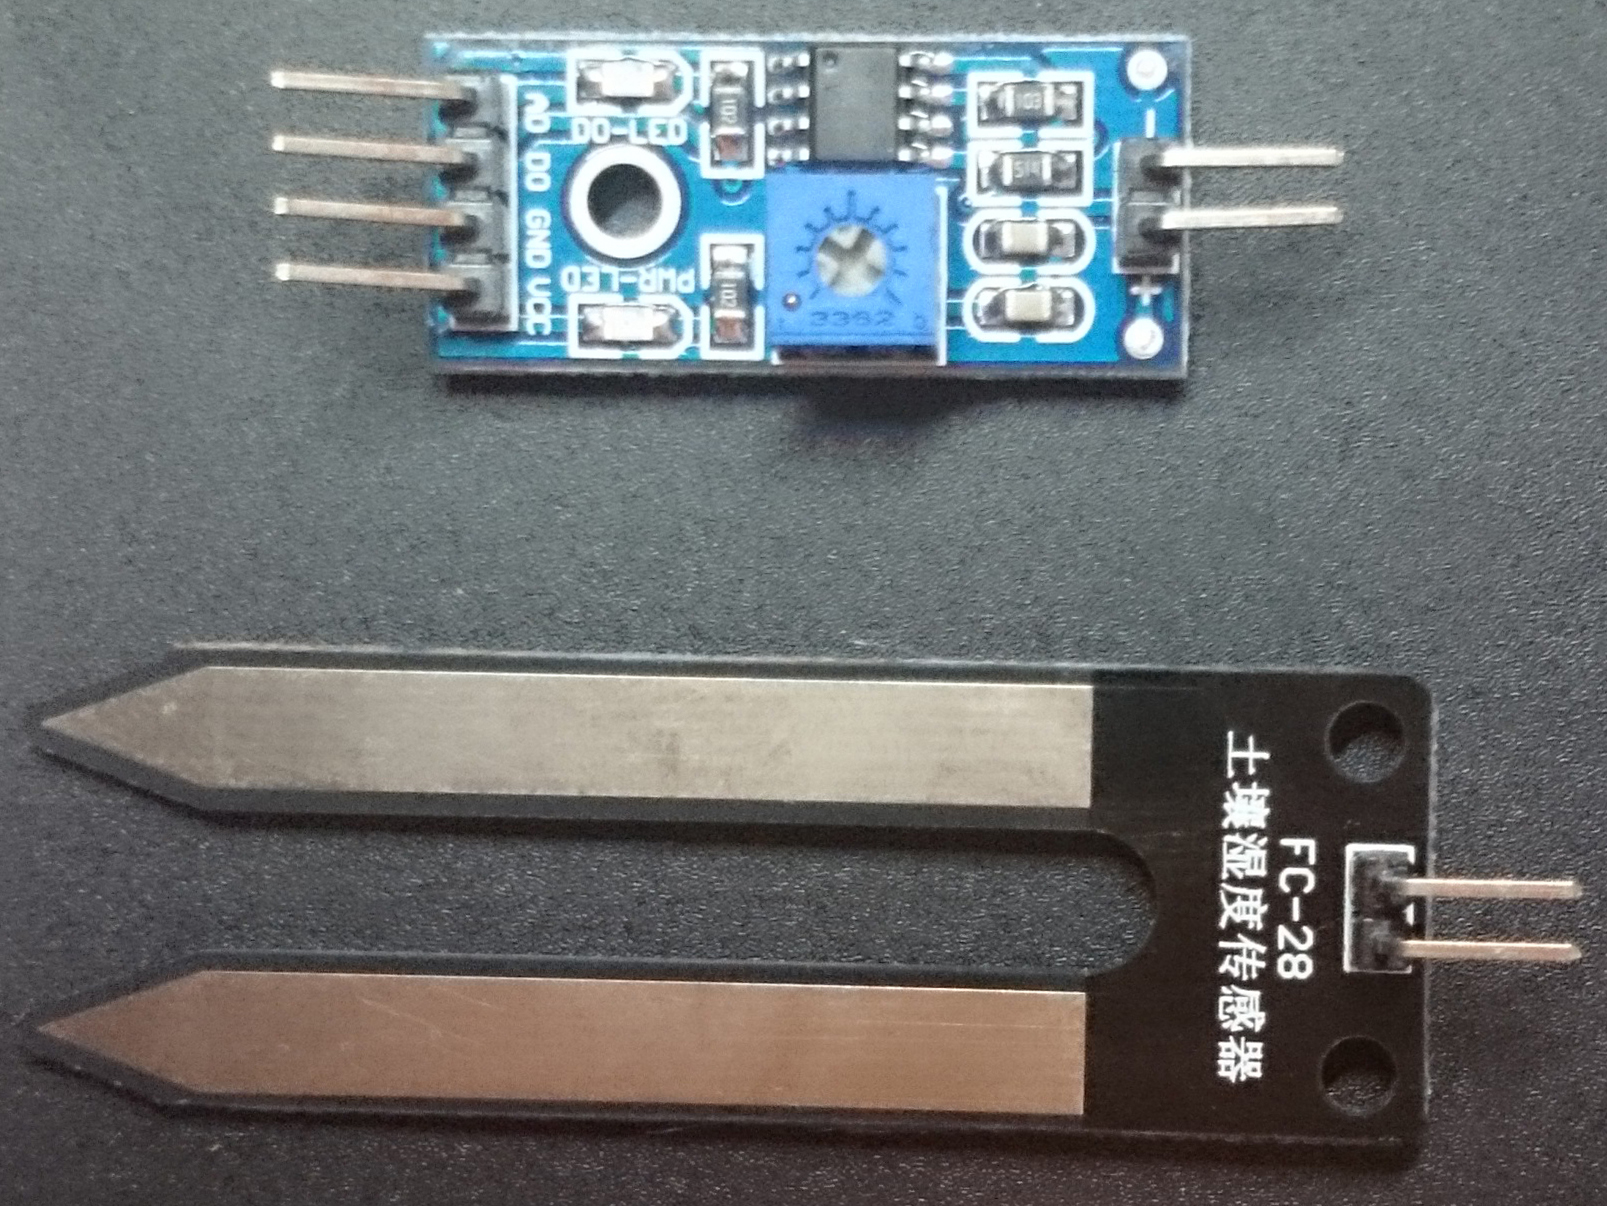
\includegraphics[width=0.8\linewidth]{bilder/_feuchteSensor1.jpg}
	\caption{Feuchtigkeitssensor mit Vorschaltung}
	\label{fig-SensorVorschaltung}
\end{figure}
Der Feuchtigkeitssensor benötigt keine weiteren Schaltelemente, da er über eine eine Vorschaltung verfügt, in der ein Spannungsteiler bereits verbaut ist. 
Abbildung \ref{fig-SensorVorschaltung} zeigt den verwendeten Sensor und die Vorschaltung. 
Es ist möglich sowohl den Analogen Wert ab-zugreifen, oder direkt eine Digitales Signal auszuwerten. Das Digitale Signal liefert einen Null-wert solange ein Grenzwiderstand nicht überschritten wird. Über ein  Potentiometer(1) lässt sich diese Grenze Einstellen. Wegen des schlechten Zugangs zum Potentiometer im eingebautem Zustand wird der Digitale Output nicht verwendet sondern der Analoge Messwert selbst ausgewertet und mit einer Variablen im Mikrocontroller abgeglichen.
		
Anpassung zu Version 1.1:
 
\begin{figure}
	\centering
	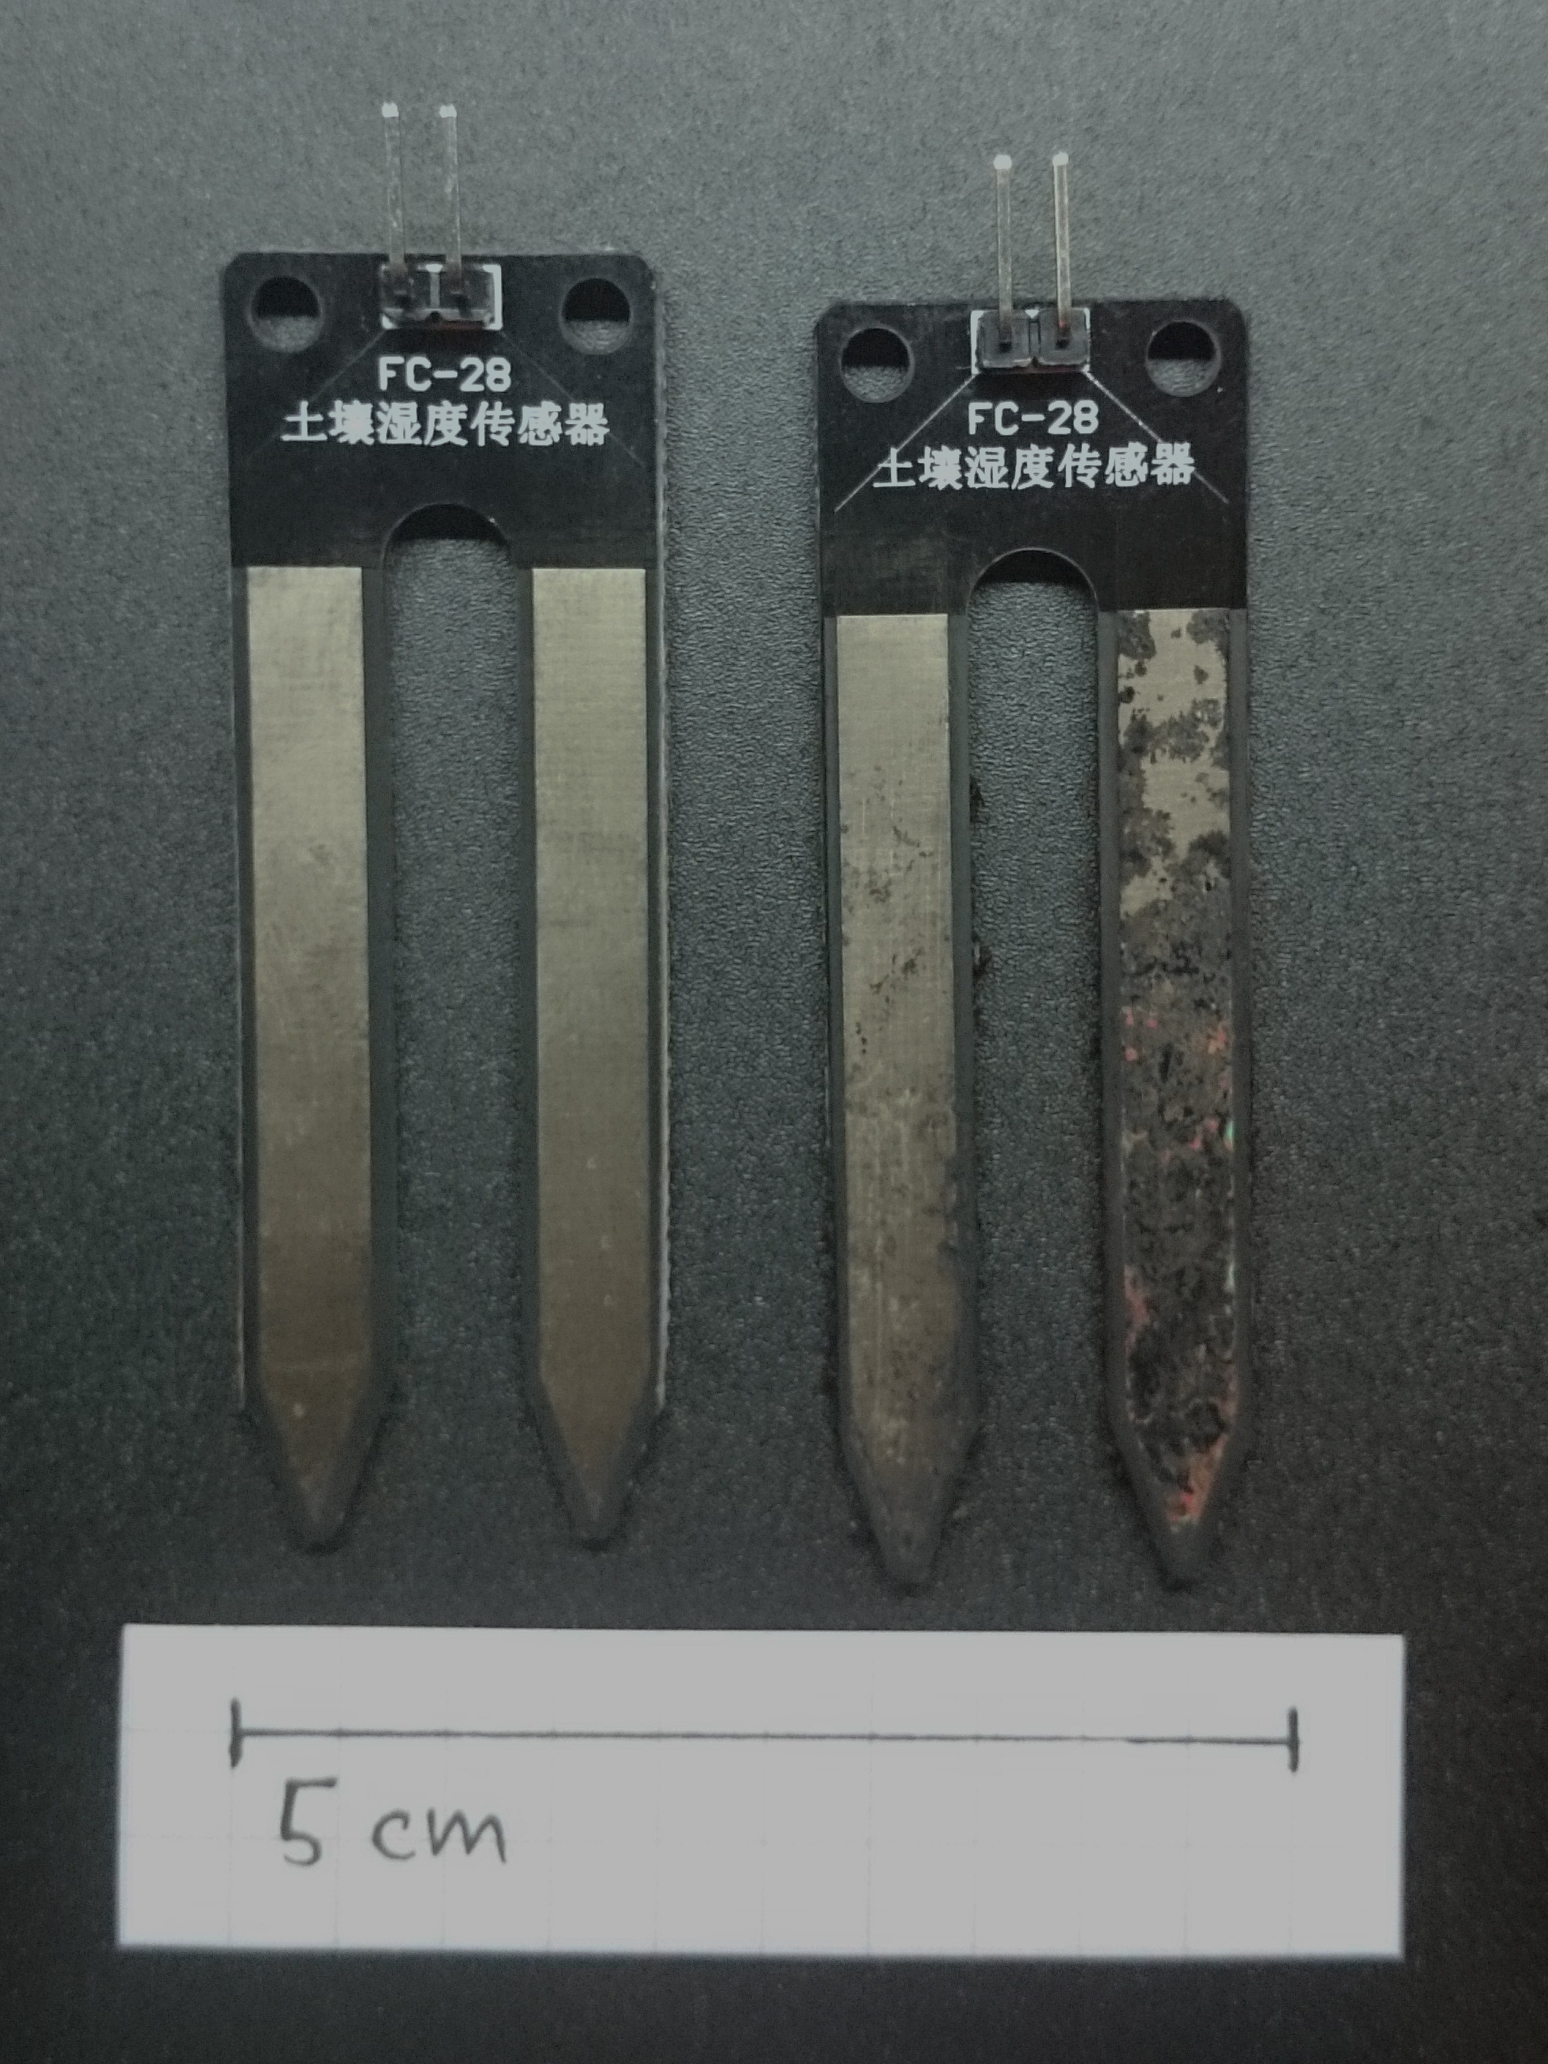
\includegraphics[width=0.8\linewidth]{bilder/_fechtesensorVergleich0.jpg}
	\caption{Vergleich neuer Sensor und Sernsor mit 48h Dauerbetrieb}
	\label{fig-SensorVergleich}
\end{figure}
Leider zeigte sich, dass nach nur 48 Stunden Dauermessung die Gabel erhebliche Korrosion erlitten hat, Abbildung \ref{fig-SensorVergleich} zeigt dies deutlich.
Die Vorschaltung sieht keine Abschaltung des Messprozesses vor noch eine Umpolung der Gabel. Deswegen muss die gesamte Vorschaltung stromlos geschaltet werden, um das Auflösen des Sensors zu verlangsamen. Hierfür haben wir für die Version 1.1 eine Transistorschaltung für den Sensor eingefügt. Über diese Schaltung wird die Vorschaltung des Feuchtigkeitssensor stromlos geschaltet. Eine Verpollung der Messgabel ist damit leider nicht möglich. Dies kann jedoch relativ einfach gelöst werden, indem der Sensor alle paar Wochen \emph{manuell} umgepolt wird. Hierfür muss lediglich die Messgabel vom Verbindungskabel abgesteckt werden und um \begin{math}180^{\circ}\end{math} gedreht wieder verbunden werden.
Beim Routing der Platine wurde die Verbindung MANUALGIES2 zu Pin 7 vergessen, weswegen diese nachträglich durch eine Drahtbrücke verbessert wurde.
	
\subsection{Stromversorgung}
Eine Stromversorgung über USB ist nicht möglich, da die Pumpe in Volllast 2,8~A benötigt. Um den Strom zu begrenzen haben wir einen \begin{math}5~\Omega\end{math} Lastwiderstand in Reihe geschallten. Die Ansteuerung der Pumpe über dem Mikrocontroller wurde über eine Transistorschaltung Gelöst (Ziffer 1 in Abbildung \ref{fig-Schaltplanv1.0}). Es ist zu überlegen, den Transistor und den Mikrocontroller über eine Schutzdiode über die Anschlüsse \emph{VENTIL-1} und \emph{VENTIL-2} vor Überspannung zu schützen, die beim abgeschaltet des gesamten Systems auftreten. Da die Pumpe jedoch nur für einen kurzen Zeitraum (Standardeinstellung 5 sekunden) in Betrieb ist, wurde davon abgesehen. 

\subsection{Kommunikation}
Ziel der Kommunikation ist es, eine Möglichkeit zu haben das Gießsystem im laufenden Betrieb einzustellen. Jede Pflanze braucht unterschiedlich viel Wasser. Genauso hat die Zusammensetzung der Erde einen Einfluss auf den gemessenen Widerstand des Feuchtigkeitssensors. Diese Werte müssen daher für jede Pflanze extra einstellbar sein. 
Wir haben uns für eine Drahtlose Kommunikation entschieden und haben uns auf den XBee Standard geeinigt. Das XBee Modul wurde direkt, d.h. ohne Verwendung eines \emph{Arduino XBEE-Shields}, mit dem Arduino verbunden. Hierfür ist es notwendig einen Pegelwandlung von 5\,V auf 3,3\,V vorzunehmen, da die Logik-Pins des XBee Moduls nicht mit 5\,V betrieben werden können. Bei dieser Pegelschaltung ist uns in Version 1.0 ein Fehler unterlaufen, weswegen wir keine Verbindung mit ein Computer aufbauen konnten. Der Fehler war, dass für die Pegelwandlung für den Anschuss TX, der Transistor falsch beschaltet wurde. Auf dem \emph{Gate} des Transistors wurde das falsche Spannungspotential geschalteten. Dieser Fehler wird für die Version 1.1 behoben und noch getestet.
\begin{figure}
	\centering
	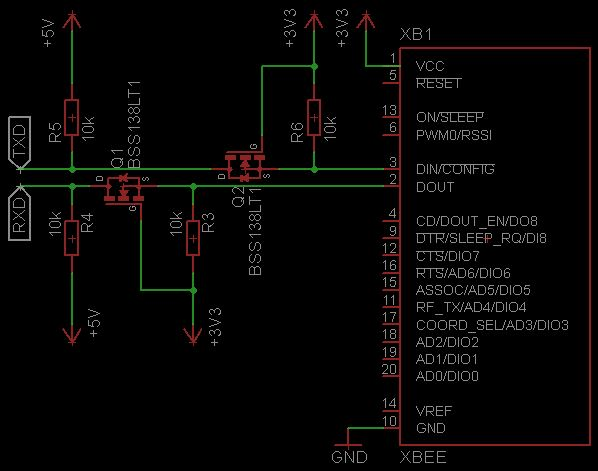
\includegraphics[width=0.8\linewidth]{bilder/v1SchaltplanXbee.jpg}
	\caption{Pegelwandler mit Small-Signal-Transistor BSS138W }
	\label{fig-Pegel}
\end{figure}


		
Die zweite Schnittstelle mit dem Menschen wird über ein Display ermöglicht. Hier lässt sich über einen Taster die einzelnen Variablen mit ihren aktuellen Werten Überprüfen. Bei dem Display Handelt es sich um ein 2 Zeiliges LCD-Display mit jeweils 16 Zeichen. Die Kommunikation zwischen Display und Mikrocontroller wird über eine I2C-Schnittstelle bewerkstelligt. Hierfür haben wir die frei verfügbare LiquidCrystal\_I2C Libary von fderbrabander verwendet.\footnote{https://github.com/fdebrabander/Arduino-LiquidCrystal-I2C-library}
		
\subsection{Mikrocontroller}
In der Version 1.0 wurde ein vorhandener Arduino Micro verwendet. Für Version 1.1 wird jedoch auf ein Arduino Nano Nachbau zurückgegriffen, da dieser im Vergleich günstiger war. Der Arduino Nano für die Version 1.1 besitzt eien ATmega168 Mikrocontroller
	
\section{Programm}
	
	\subsection{Mikrocontroller}
	Die Aufgaben des Mikrocontrollers sind die folgenden:
		\begin{itemize}
			\item Messung der Feuchtigkeit
			\item Messung der Helligkeitssensor
			\item Vergleich der Messwerte mit den festgelegten Grenzen
			\item Ansteuerung der Pumpensystem
			\item Ausgabe der wichtigen Variablen auf dem Display über Taster
			\item Manuelles Gießen über Taster
			\item Display Hintergrundbeleuchtung abschalten nach 60  Sekunden
			\item Übertragen/Empfangen von Einstellungen über xBee Verbindung
		\end{itemize}
		
	In der ersten Version wurden die Messungen andauernd durchgeführt. Wie aber bereits oben erläutert hat dies zu einer starken Korrosion am Feuchtigkeitssensor geführt. Aus diesem Grund wurde für die Version 1.1 einige Änderungen eingeführt. Anstelle bei jedem Aufruf der Loop() Methode eine Messung durchzuführen wird nur noch alle 4 Stunden eine Messung vorgenommen. Ist das Intervall abgelaufen wird der Feuchtigkeitssensor über eine Transistorschaltung angeschaltet und anschließend ausgelesen. Dadurch ist der Sensoren nur noch für einen kurzen Zeitraum unter Strom, was die Lebensdauer des Feuchtigkeitssensor verlängert.
		
	
	\subsection{Setuptool}
	Da die Erde in jeder Pflanze eine andere Zusammensetzung hat und jede Pflanze unterschiedlich viel Wasser benötigt ist es notwendig die Grenzwerte für die Feuchtigkeit und die Wassermenge einzustellen. Hierfür gibt es ein Cmd-Tool welches über die 
	
\section{Sparversion}
	In der der günstigeren Variante der Gießanlage wurde alles, wurde die Konstruktion auf das wesentlichste beschränkt,das Gießen.
	\subsection{Aufbau}
	In dieser Version wird auf das Display und die Kommunikation verzichtet.
	
	\subsection{Logik}
	Um weiter Stromsparen zu können wurde diese Version nicht mit Arduino, sondern mit C programmiert.
	Dies ermöglicht die Ausnutzung der Sleep Modi und die Interrupts des ATMega328. 
	Dadurch befindet sich der \glqq Arduino Nano\grqq \ hauptsächlich im Schlafmodus und verbraucht deutlich weniger Energie. 
	
\section{BOM - Bill of Matirial}
	
	\section{Kostenplan}
	
	\section{Resüme - Do's And Dont's}	


\end{document}


